\documentclass[preview,border=2pt]{standalone}
\usepackage{pgfplots}
\pgfplotsset{compat=1.18}
\usepgfplotslibrary{patchplots}
\usetikzlibrary{patterns}
\usepackage{xcolor}

\begin{document}

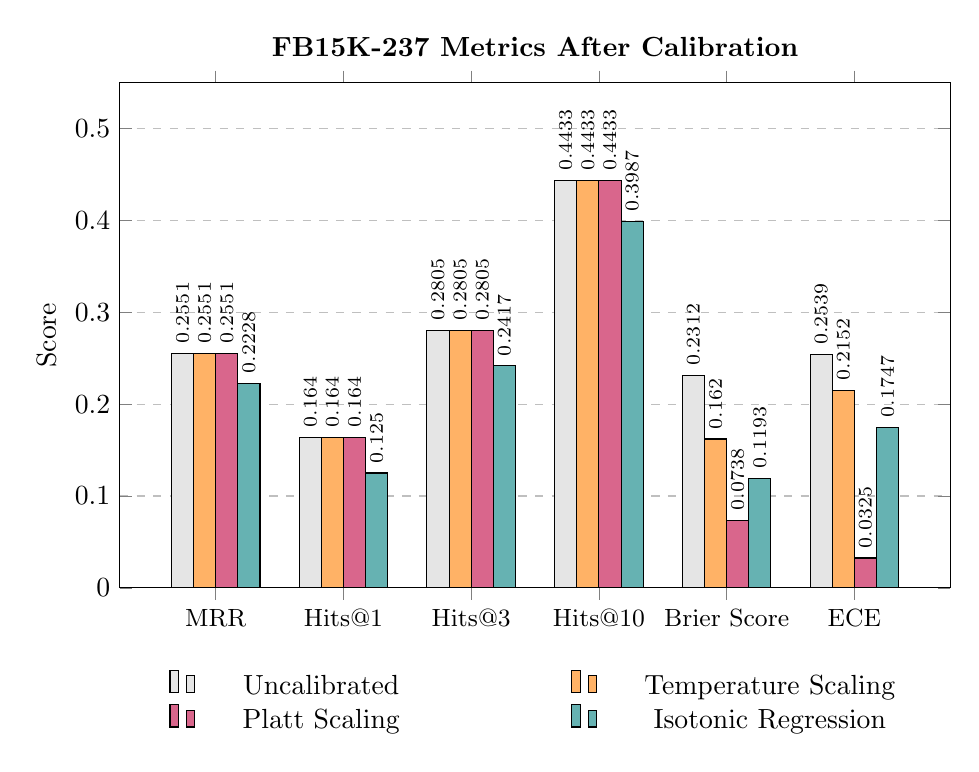
\begin{tikzpicture}
    \begin{axis}[
        ybar=0pt,
        title={\textbf{FB15K-237 Metrics After Calibration}},
        width=\textwidth,
        height=8cm,
        symbolic x coords={MRR, Hits@1, Hits@3, Hits@10, Brier Score, ECE},
        xtick=data,
        nodes near coords,
        nodes near coords style={font=\scriptsize, rotate=90, anchor=west, /pgf/number format/fixed, /pgf/number format/precision=4},
        ymin=0, ymax=0.55,
        ylabel={Score},
        ymajorgrids=true,
        grid style=dashed,
        bar width=8pt,
        enlarge x limits=0.15,
        legend style={at={(0.5,-0.15)}, anchor=north, legend columns=2, column sep=15pt, /tikz/every even column/.append style={column sep=60pt}, draw=none},
        xticklabel style={font=\small},
    ]
    
    % Uncalibrated
    \addplot[pattern=crosshatch, pattern color=gray!70, fill=gray!20, draw=black] coordinates {
        (MRR, 0.2551)
        (Hits@1, 0.1640)
        (Hits@3, 0.2805)
        (Hits@10, 0.4433)
        (Brier Score, 0.2312)
        (ECE, 0.2539)
    };
    
    % Temperature Scaling
    \addplot[fill=orange!60!white, draw=black] coordinates {
        (MRR, 0.2551)
        (Hits@1, 0.1640)
        (Hits@3, 0.2805)
        (Hits@10, 0.4433)
        (Brier Score, 0.1620)
        (ECE, 0.2152)
    };
    
    % Platt Scaling
    \addplot[fill=purple!60!white, draw=black] coordinates {
        (MRR, 0.2551)
        (Hits@1, 0.1640)
        (Hits@3, 0.2805)
        (Hits@10, 0.4433)
        (Brier Score, 0.0738)
        (ECE, 0.0325)
    };
    
    % Isotonic Regression
    \addplot[fill=teal!60!white, draw=black] coordinates {
        (MRR, 0.2228)
        (Hits@1, 0.1250)
        (Hits@3, 0.2417)
        (Hits@10, 0.3987)
        (Brier Score, 0.1193)
        (ECE, 0.1747)
    };

    \legend{Uncalibrated, Temperature Scaling, Platt Scaling, Isotonic Regression}
    \end{axis}
\end{tikzpicture}

\end{document}